\chapter{Development}
\label{ch:development}
%Este capítulo é parte principal do trabalho acadêmico e deve conter a exposição ordenada e detalhada do assunto.
%Divide-se em seções e subseções, em conformidade com a abordagem do tema e do método, abrangendo:
%revisão bibliográfica, materiais e métodos, técnicas utilizadas, resultados obtidos e discussão.
Distributed reinforcement learning (RL) has evolved considerably in response to the demands of complex tasks such as game playing and financial trading.
Early methods such as the Asynchronous Advantage Actor-Critic (A3C)
algorithm introduced the concept of multiple parallel workers collecting experiences independently,
which helped to reduce update variance and speed up training.
Building on these ideas, architectures like IMPALA and Gorila have decoupled data collection from model training by using
a decentralized learner and worker structure, which periodically synchronizes the policy with the updated gradient
from the workers through gradient passing.
This design enables significant scalability across heterogeneous computing resources and facilitates high-throughput training.

As mentioned in \fullref{ch:introduction}, a key challenge present in these systems is the communication overhead incurred when transmitting experiences or
updated policies between the learner and the workers.
The IMPALA algorithm aggregates trajectories from multiple workers into
batches for efficient gradient computation while managing the staleness of policy information.
More recent approaches, such as SEED RL, have further optimized communication by bundling inference with training updates.
This reduces the latency associated with model parameter transmission and minimizes network congestion, thereby improving overall training efficiency.
In parallel, methods like Ape-X have introduced distributed prioritized experience replay, where critical experiences are sampled with higher probability,
enhancing data efficiency in scenarios where high-frequency data generation is crucial.

In the context of financial applications, RL environments often integrate realistic market simulators.
These simulators statistically represent stylized facts of limit order book (LOB), which are discussed
further in \fullref{subsec:environment}.
For such simulators, the distributed architecture must handle not only the high throughput of simulation data but also the
precise timing of order execution and asynchronous policy updates.
This thesis builds upon existing distributed algorithms through means of shared parallel environments,
designed specifically to address the nature of high-frequency trading applications.
In the following sections, we present the design and implementation of our proposed architecture,
which we refer to as Parallel Environments for Asynchronous Reinforcement Learning (PEARL).

\section{Literature Review}
\label{sec:literature_review}

We performed a simple overview of recent literature regarding distributed reinforcement learning,
and categorized the results according to groups of tags.
This review was made with the purpose of highlighting frequently used algorithms, RL metrics,
and types of system and network benchmarks.
To gather relevant literature, we searched the Web of Science database using the following search query,
while limiting the results to the last 5 years:

\begin{verbatim}
    ALL=(
        (
            "distributed" OR "parallel" OR
            "multi-agent" OR "asynchronous"
        )
        AND
        (
            "shared environments" OR "replay buffer" OR
            "trajectory sampling" OR "experience sampling"
        )
        AND "reinforcement learning"
    )
\end{verbatim}

Initially, a total of 68 papers matched the search query, with 34 being deemed unfit or irrelevant to the
present research question.
The bibliography analysis refeers to the remaining 33, where the tagged categories are as shown:

\begin{itemize}[leftmargin=*, label={--}]
    \item \textbf{Algorithm Categories} (e.g., Q-learning, Actor-Critic, Policy Gradients)
    \item \textbf{Learning Paradigm} (On-Policy, Off-Policy, Model-Free, Model-Based)
    \item \textbf{Communication Model} (Centralized, Decentralized, Asynchronous, Synchronous)
    \item \textbf{RL Metrics} (Reward, Sample Efficiency, Convergence, Stability)
    \item \textbf{System Metrics} (Wall Speed, Latency, Memory, Core Efficiency)
\end{itemize}



\section{Environment and Agent Methodology}
\label{sec:methodology}

As mentioned in \fullref{ch:introduction}, the proposed PEARL framework enables multiple RL agents (workers)
to share a single environment instance rather than running isolated simulations and thus
minimize redundant computations and communication overhead typically
encountered when synchronizing separate environment instances.
The dynamics of the simulator and the implemented agent used for testing the framework are described in the following subsections.

%! Author = rzimmerdev
%! Date = 3/28/25

% Preamble
\documentclass[11pt]{article}

% Packages
\usepackage{amsmath}
\usepackage{graphicx}

% Document
\begin{document}
    \subsection{Simulated Trading Environment and Limit Order Book Dynamics}
    \label{subsec:environment}
    The simulated environment is designed to replicate key aspects of a modern financial market by incorporating a limit order book (LOB) mechanism.
    A LOB is the core structure in many electronic trading systems, where buy and sell orders are organized by price and time priority,
    thereby reflecting the real-time supply and demand of an asset.

    In this environment, agents interact with the market by submitting orders that represent their actions.
    Specifically, each action corresponds to placing a limit order—a directive to buy or sell a specified quantity at a predetermined price.
    When an agent submits an order, it is added to the appropriate side of the LOB, where orders are queued according to their price and
    the time at which they were submitted.
    An order is executed if there is a matching order on the opposite side of the book that satisfies the price condition;
    otherwise, it remains in the book until a suitable counter-order appears or the order is cancelled by the agent.
    This event-driven process mimics the intricate dynamics of order matching observed in real markets.

    The simulation employs a discrete-event framework to model these processes accurately.
    At each simulation step, the environment generates an observation that includes critical details such as the best bid and ask prices,
    the order book depth across various price levels, and records of recent trade executions.
    These observations are then provided to the agents, enabling them to update their strategies based on the evolving market state.

    Order submission and execution in the simulated environment are handled asynchronously.
    Agents send their orders via a messaging layer—implemented with a high-performance protocol like
    ZeroMQ—to ensure that multiple agents can interact with the shared LOB concurrently without incurring significant delays.
    This asynchronous architecture not only improves simulation throughput but also closely aligns with
    the latency-sensitive nature of high-frequency trading environments.

    By integrating a realistic LOB into the simulation, the environment provides a robust testbed for exploring how
    distributed reinforcement learning algorithms can learn and adapt in complex, dynamic markets.
    The detailed representation of market microstructure, combined with the precise handling of order events,
    allows for rigorous scientific investigation into the interplay between order submission strategies and market behavior.

    \begin{figure}[htb]
        \centering
        \includegraphics[width=0.8\textwidth]{img/lob.png}
        \caption{Visualization of a limit order book (LOB) with buy and sell orders organized by price and time priority.}
        \label{fig:lob}
    \end{figure}

    The system dynamics are modeled as a continuous-time Markov Decision Process (MDP), where the transition probabilities
    \( P(s', t|s, a) \) are governed by the Kolmogorov forward equation:

    \[
        \frac{\partial P(s', t|s, a)}{\partial t} = \int_S L(x|s, a, t) P(s'|x, a, t) \, dx
    \]

    Here, \( a \) represents the action chosen by the control agent according to a policy \( \pi(s) \), and \( L(x|s, a, t) \) is the generator operator,
    which defines the dynamics of state transitions at any given time \( t \).
    Solving for the transition probabilities is often approached either analytically through closed-form solutions,
    as in earlier works (Avellaneda et al., 2008; Gueant et al., 2017),
    or numerically via approximations (e.g., by simulating trajectories or using reinforcement learning methods).

    The market-making problem is modeled using online reinforcement learning, where the simulator represents a
    limit order book (LOB) that reflects stylized market behaviors.
    The event timing in the LOB follows a Hawkes process, capturing the self-exciting nature of clustered order arrivals.
    The intensity \( \lambda(t) \) of this process evolves as:

    \begin{gather*}
        \lambda(t) = \mu + \sum_{t_i < t} \phi(t - t_i)\\
        \phi(t - t_i) = \alpha e^{-\beta(t - t_i)}\\
    \end{gather*}

    where \( \mu > 0 \) is the baseline intensity, and \( \alpha \), \( \beta \) govern the magnitude and decay of past events' influence.
    Bid and ask prices are modeled as separate Geometric Brownian Motion (GBM) processes, with prices evolving according to:

    \begin{gather*}
        dX_{\text{ask}} = (\mu_t + s_t) X_{\text{mid}} \, dt + \sigma dW_t\\
        dX_{\text{bid}} = (\mu_t - s_t) X_{\text{mid}} \, dt + \sigma dW_t\\
    \end{gather*}

    where \( \mu_t \) is the drift, \( s_t \) is the spread, and \( \sigma \) is the volatility.
    The drift \( \mu_t \) follows a mean-reverting Ornstein-Uhlenbeck process, while the spread \( s_t \) follows a Cox-Ingersoll-Ross process,
    ensuring a positive spread.
    The midprice \( X_{\text{mid}} \) is calculated as the average of the current bid and ask prices:

    \[
        X_{\text{mid}} = \frac{X_{\text{ask}} + X_{\text{bid}}}{2}
    \]

    In the absence of orders, the midprice is based on the last traded price or an initial value.
    Price volatility is modeled using a GARCH(1,1) process:

    \[
        \sigma_t^2 = \omega + \alpha \epsilon_{t-1}^2 + \beta \sigma_{t-1}^2
    \]

    where \( \sigma_t \) is the volatility, \( \epsilon_{t-1} \) is the return shock, and \( \alpha \), \( \beta \) are parameters capturing volatility clustering.
    Order quantities \( q_{\text{ask}} \) and \( q_{\text{bid}} \) are modeled as Poisson random variables with arrival rate \( \lambda_q \),
    reflecting stochastic order arrivals.
    The simulator is implemented using a Red-black tree structure for the LOB, and all market regime variables (e.g., spread, order arrival rate, and price drift)
    are sampled from predefined distributions and inserted into the system at each event time step.


\end{document}
%! Author = rzimmerdev
%! Date = 3/28/25

% Preamble
\documentclass[11pt]{article}

% Packages
\usepackage{amsmath}
\usepackage{amsfonts}

% Document
\begin{document}
    \subsection{Chosen Agent Architecture}
    \label{sec:agent}

    The reinforcement learning problem is formulated as a Markov Decision Process (MDP) with a state space \( S \),
    action space \( A \), transition probabilities \( P(s'|s, a) \), and rewards \( R(s, a) \).
    The underlying goal is to learn a policy \( \pi \) that maximizes the expected return over time.

    In reinforcement learning, the Bellman equation recursively defines the value of a state, \( V(s) \),
    in terms of the reward and the expected future state values.
    For a given policy \( \pi \), the Bellman equation for the value function \( V^{\pi}(s) \) is:

    \[
        V^{\pi}(s) = \sum_{a \in A} \pi(a|s) \sum_{s' \in S} P(s'|s, a) \left( R_t + \gamma V^{\pi}(s') \right)
    \]

    where \( R_t \) is the reward at time \( t \), and \( \gamma \) is the discount factor.
    The goal is to find the optimal policy \( \pi^* \) that maximizes the expected return, which is given by:

    \[
        V^*(s) = \max_a \mathbb{E}[R_t + \gamma V^*(s') | s = s, a = a]
    \]

    Policy iteration and value iteration are methods to solve this equation, but they become computationally expensive for large state spaces.
    In such cases, neural networks are used to approximate the value function or the policy itself, making them suitable for complex environments.
    The Generalized Policy Iteration is a framework that unifies these methods by iteratively evaluating and improving the policy.
    Most modern reinforcement learning algorithms and the current state-of-the-art methods are based on this framework,
    including but not limited to Q-learning, Actor-Critic (and variations), and Policy Gradient methods.

    % diagrams/gpi.pdf
    \begin{figure}[htb]
        \centering
        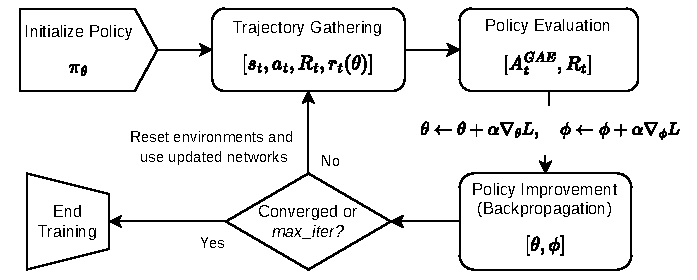
\includegraphics[width=0.8\textwidth]{diagrams/gpi.pdf}
        \caption{Generalized Policy Iteration (GPI) diagram for Policy Gradient methods.}
        \label{fig:gpi}
    \end{figure}

    Policy Gradient methods are particularly well-suited for continuous action spaces and have been widely used in finance and trading applications.
    The approach involves parameterizing the policy \( \pi_\theta(a|s) \) with a neural network and optimizing it directly to maximize the expected return.
    The policy gradient given a state-action pair \( (s, a) \) and policy network \( \pi_\theta \) is:

    \[
        \nabla_\theta J(\theta) = \mathbb{E}_{\tau \sim \pi_\theta} \left[ \sum_{t=0}^{T} \nabla_\theta \log \pi_\theta(a_t | s_t) A^\pi(s_t, a_t) \right]
    \]

    For Proximal Policy Optimization (PPO), the policy update is constrained to prevent excessive changes by using a clipped surrogate objective:

    \[
        L_{\text{actor}}(\theta) = \mathbb{E}_t \left[ \min \left( r_t(\theta) \hat{A}_t, \text{clip}(r_t(\theta), 1-\epsilon, 1+\epsilon) \hat{A}_t \right) \right]
    \]

    where \( r_t(\theta) \) is the probability ratio between the new and old policies, and \( \hat{A}_t \) is the advantage function.
    The critic loss is:

    \[
        L_{\text{critic}} = \mathbb{E}_t \left[ (V(s_t) - R_t)^2 \right]
    \]

    These updates are performed iteratively, using a neural network with backpropagation to minimize the loss and improve the policy.
    PPO ensures stability by limiting the policy update size.

    To benchmark the agent, we use a closed-form expression for the optimal bid-ask spread, as proposed by Avellaneda et al. (2008):

    \[
        \delta^* = \sigma \sqrt{2} \, \text{erf}^{-1} \left( \frac{1}{2} \left( 1 + \frac{\mu}{\sigma} \right) \right)
    \]

    where \( \sigma \) is the volatility, \( \mu \) is the mean spread, and \( \text{erf}^{-1} \) is the inverse error function.
    The optimal bid-ask spread pair is then:

    \[
        p_{\text{bid}} = \mu - \delta^*, \quad p_{\text{ask}} = \mu + \delta^*
    \]

    This closed-form expression serves as a simpler model to compare the agent's performance against a more complex environment.

    \begin{figure}[htb]
        \centering
        \includegraphics[width=0.8\textwidth]{diagrams/policy.pdf}
        \caption{Architecture of the reinforcement learning agent used in the simulation.}
        \label{fig:agent}
    \end{figure}

\end{document}

\section{Technical Details and Framework Description}
\label{sec:technical_details}

%! Author = rzimmerdev
%! Date = 3/28/25

% Preamble
\documentclass[11pt]{article}

% Packages
\usepackage{amsmath}

% Document
\begin{document}
    \subsection{Parallel Environments for Asynchronous Reinforcement Learning (PEARL)}
    \label{subsec:pearl}
    The proposed architecture builds on the core idea of sharing a single, highly parallel environment among multiple agents while
    maintaining an efficient and scalable actor–learner framework.
    In contrast to conventional distributed reinforcement learning systems—where each worker simulates an independent environment instance—
    the shared environment paradigm leverages a unified simulation that is concurrently accessed by multiple workers.
    This design minimizes redundant computations and memory overhead,
    which is especially critical in high-frequency trading simulations where the fidelity and speed of the limit order book (LOB) dynamics are paramount.

    At the heart of the architecture lies a central learner that manages the global policy.
    Upon initialization, the learner spawns several worker processes using Python's multiprocessing library.
    Each worker retrieves the latest version of the shared policy and uses it to interact with the common environment.
    In this setup, workers act as both data collectors and order executors: they send orders (actions) to the LOB simulation,
    receive market updates, and construct trajectories that capture the sequence of states, actions, and rewards.
    By sharing the environment, workers benefit from a consistent and synchronized view of the simulated market,
    which enhances the quality of the experience data collected.

    Communication between the learner and workers is designed to be asynchronous.
    Workers submit their generated trajectories to the learner via a high-performance messaging layer implemented with ZeroMQ\@.
    This asynchronous mechanism enables workers to operate independently—without waiting for policy updates—
    thereby reducing idle time and mitigating the staleness issues often encountered in distributed setups

    % graphics for diagrams/pearl_architecture.pdf
    \begin{figure}[htb]
        \centering
        \includegraphics[width=0.8\textwidth]{diagrams/pearl_architecture.pdf}
        \caption{Overview of the Parallel Environments for Asynchronous Reinforcement Learning (PEARL) framework.}
        \label{fig:pearl_architecture}
    \end{figure}

    Meanwhile, the learner continuously processes incoming trajectories from the workers, updates the global policy using reinforcement learning algorithms,
    and the workers can call the shared agent parameters at any time.
    This cycle ensures that while each worker may temporarily operate on slightly outdated policy parameters,
    the overall system converges steadily as fresh data are incorporated into the learner's updates.

    By allowing the workers to share a common environment and asynchronously update the global policy,
    the proposed architecture aims to strike a balance between computational efficiency and learning performance.
    The computational load—especially during intensive simulations and gradient computations—is balanced effectively
    across the workers, due to the pooled resource utilization.
    The worker pool design also contributes to reducing the overall system latency,
    as workers can operate and unlock their individual threads while waiting for the environment to synchronize other agents and return a new state.
    In traditional architectures, the cost of transferring model parameters and simulation data between isolated environment instances can introduce significant delays.
    By contrast, our approach minimizes such overhead by centralizing the learner weights and leveraging efficient, low-latency communication channels.
    This architecture is particularly well-suited for real-time applications, such as high-frequency trading,
    where even minor delays can adversely affect performance.

    In summary, this integrated system architecture—comprising a shared simulation environment, an asynchronous actor–learner framework, and
    a robust communication backbone—addresses many of the limitations inherent in earlier distributed reinforcement learning approaches.
    By combining the advantages of shared resource utilization with scalable, asynchronous updates, the architecture provides a solid foundation for
    developing reinforcement learning systems capable of operating effectively in complex, dynamic domains.

    \begin{figure}
        \centering
        \includegraphics[width=0.8\textwidth]{diagrams/pipeline.pdf}
        \caption{Illustration of the pipeline between learners, their workers and a single environment instance.}
        \label{fig:lob_simulation}
    \end{figure}


\end{document}
%! Author = rzimmerdev
%! Date = 3/28/25

% Preamble
\documentclass[11pt]{article}

% Packages
\usepackage{amsmath}

% Document
\begin{document}
    \subsection{Communication Protocols and Network Layout}
    \label{subsec:communication}

    \begin{figure}[htb]
        \centering
        \includegraphics[width=0.5\textwidth]{diagrams/service_mesh}
        \caption{Overview of the service mesh architecture for communication between agents and the central learner.}
        \label{fig:service_mesh}
    \end{figure}

    The communication infrastructure of the system is designed to support fully asynchronous interactions
    between distributed actors and the centralized learner module.
    The adopted service mesh architecture, shown in~\autoref{fig:service_mesh}, provides logical separation between communication and computation concerns,
    and allows the learner and environment subsystems to scale independently across compute nodes.

    As previously discussed, we employ a brokerless ZeroMQ Router/Dealer pattern for the messaging layer.
    This setup enables direct point-to-point communication between actors and the learner without requiring intermediate brokers or persistent queues,
    minimizing the round-trip time of trajectory and gradient message exchange.
    ZeroMQ's non-blocking I/O capabilities and lock-free shared memory buffers make it suitable for high-frequency,
    low-latency applications such as algorithmic trading environments.

    Each actor maintains an independent outbound socket pool for pushing trajectory segments or parameter update requests to the learner.
    This decouples action inference and experience collection from the learning pipeline,
    allowing learners to continuously receive and process incoming batches even in the presence of straggler workers.
    Moreover, actors are not synchronized globally; the system is designed so that each actor proceeds independently through environment interaction,
    buffering experience locally before asynchronously committing the collected data to the learner.

    \begin{figure}[htb]
        \centering
        \includegraphics[width=0.8\textwidth]{diagrams/communication}
        \caption{Communication flow between agents and the central learner using ZeroMQ messaging.}
        \label{fig:communication}
    \end{figure}

    \autoref{fig:communication} illustrates the end-to-end communication pipeline.
    Each agent is initialized with a direct messaging channel to the central learner process.
    The learner operates as a multiplexed ZeroMQ Router endpoint capable of concurrently handling multiple inbound streams.
    It tags incoming messages with agent identifiers and manages per-agent buffers for temporal ordering and batching of updates.
    This enables efficient mini-batch construction for training while preserving per-agent data locality when needed.

    The overall communication design maximizes concurrency while controlling the negative effects of different processing speeds per agent.
    Since the communication layer is built on top of a service mesh,
    it also supports horizontal scaling by adding agents without need for centralized coordination,
    as both learners and environments can be shutdown, restarted and added without interfering with training.
    This is a key design goal for large-scale reinforcement learning in latency-sensitive domains such as market making and high-frequency trading,
    where simulation fidelity, throughput, and data freshness all interact to determine the agent’s learning efficiency and performance.

\end{document}
